\section{El problema del viajante de comercio}

\begin{frame}{Problema}
Hallar el recorrido con distancia mínima en un conjunto de
ciudades que pase por todas las ciudades y regrese al punto inicial.

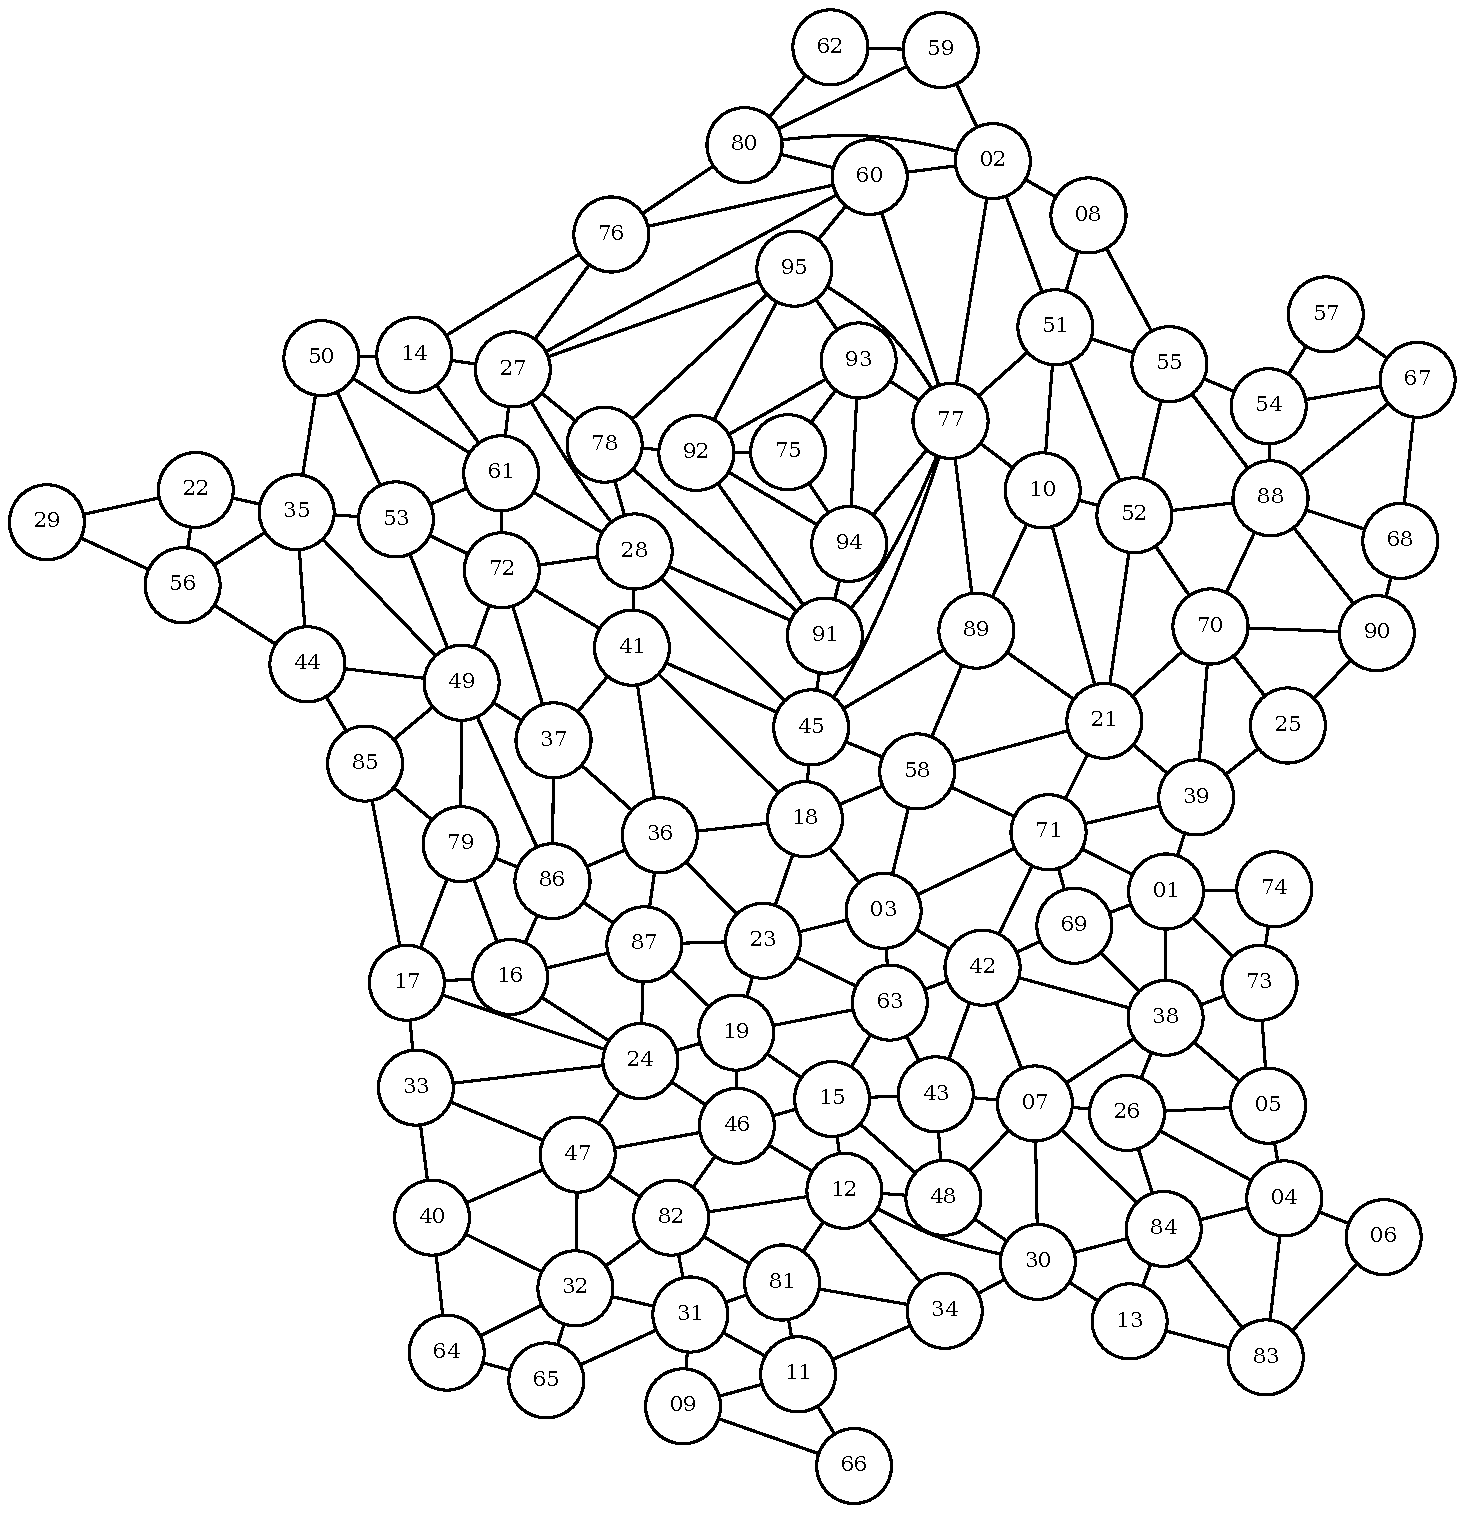
\includegraphics[width=.5\textwidth]{img/Francia} \centering
\end{frame}

\begin{frame}{Algoritmos}
\begin{description}
 \item[Entrada:] Ficheros con ciudades indicadas como puntos en el plano según sus
 coordenadas.
 \item[Salida:] \texttt{vector<int>} con el orden en el que se recorren las ciudades.
\end{description}
\end{frame}

% TODO: todo lo posterior